\documentclass[margin=0.5mm]{standalone}
\usepackage{pgfplots}
\usetikzlibrary{pgfplots.groupplots}
\pgfplotsset{compat=1.7}
\definecolor{BoxCol}{rgb}{0.43,0.62,0.86}

\begin{document}
	\thispagestyle{empty}
	
%	\begin{figure}[t]
%		\centering
		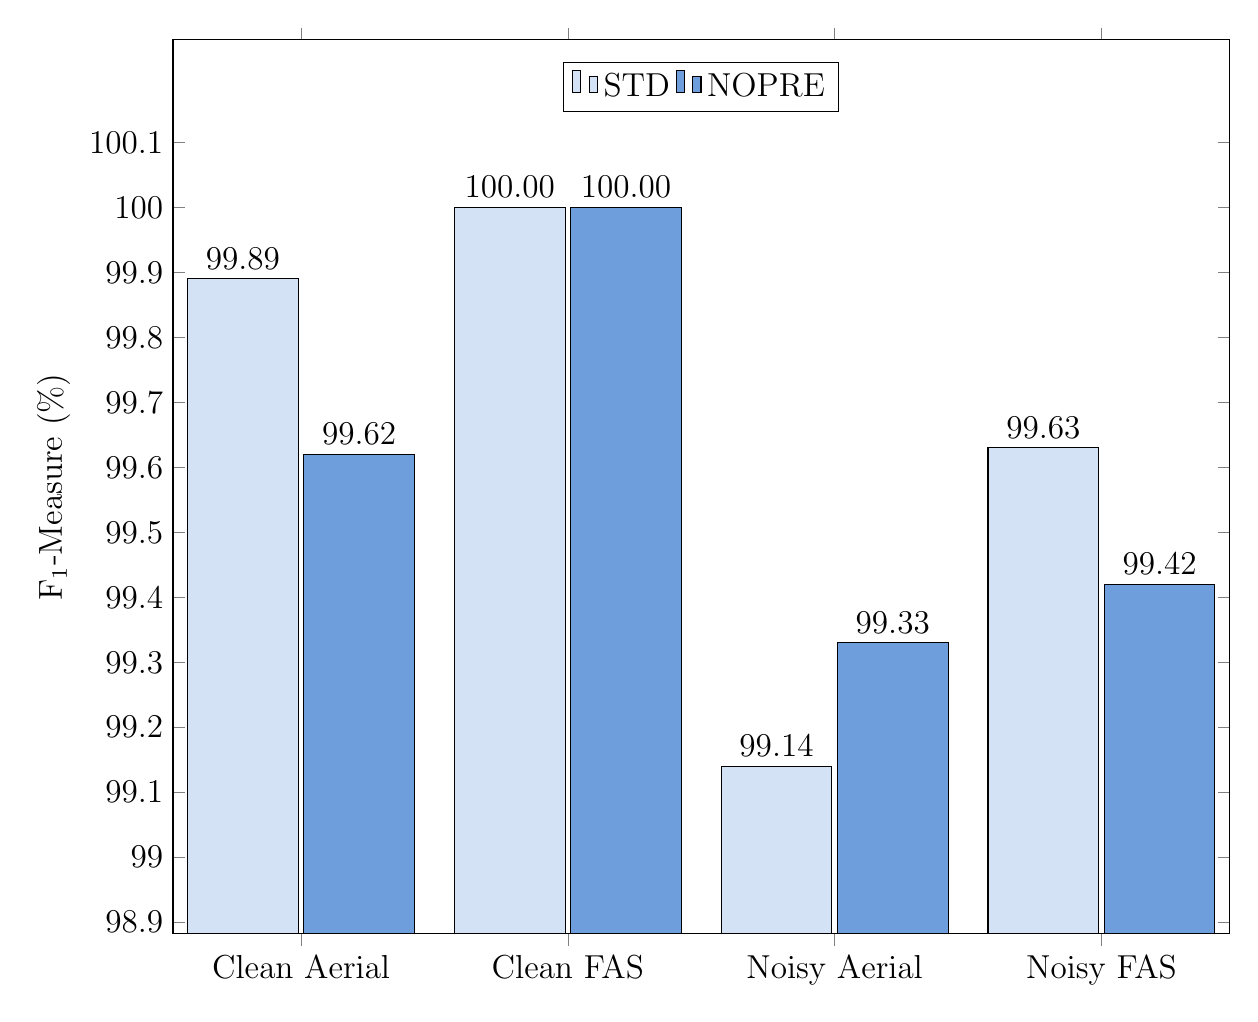
\begin{tikzpicture}
		\begin{axis}[
		width=15cm,
		enlarge x limits=0.16,
		enlarge y limits=0.3,
		%enlargelimits=true,
			ybar,
			%legend style={at={(0.5,-0.15)},
			legend style={at={(0.5,0.975)},
			anchor=north,legend columns=-1},
			ylabel={F$_1$-Measure (\%)},
			symbolic x coords={Clean Aerial,Clean FAS,Noisy Aerial,Noisy FAS},
			xtick=data,
			nodes near coords={\pgfmathprintnumber[fixed zerofill, precision=2]{\pgfplotspointmeta}},
			nodes near coords align={vertical},
			bar width=40pt,
			style={font=\large},
			ytick={98.0,98.1,...,100.1},
			ymax=100
		]
		%						STD		NPRE	
		%			Aerial
		%				Clean	99.89	99.62	
		%				Noisy   99.14	99.33
		
		%			FAS		
		%				Clean	100 	100 	
		%				Noisy   99.63	99.42	
		
		
		\addplot [color=black,fill=BoxCol!30!white] coordinates {(Clean Aerial,99.89) (Clean FAS,100) (Noisy Aerial,99.14) (Noisy FAS,99.63) };
		\addplot [color=black,fill=BoxCol!100!white] coordinates {(Clean Aerial,99.62) (Clean FAS,100) (Noisy Aerial,99.33) (Noisy FAS,99.42)};		

%		\addplot [color=black,fill=darkgray] coordinates {(NA,99.14) (NF,99.63)  };
%		\addplot [color=black,fill=lightgray] coordinates {(NA,99.33) (NF,99.42) };	
		
		\legend{STD,NOPRE}
		\end{axis}
		\end{tikzpicture}
		
		%\vspace{-0.7cm}
		%\caption{Left: the pitch distribution for the 10 male speakers. Right: the active speech level for the 20 speakers.}\label{fig:pitch}
		%\vspace{-0.5cm}
%	\end{figure}
\end{document}